
\chapter{Implementation}
\label{Implementation}

\section{Early Development}
After the first weeks where background reading were done and designing a plan for the final program, work using the Webots\textsuperscript{\texttrademark} simulator was started. \\ More information about the different stages can be found in the following sub-sections. 

\subsection{Webots Tutorials}
In the beginning different tutorials and demo following  programs included in the Webots installation were followed. 
This helped to see how the simulator works, what it can do and what possibilities the Webots API gives an developer. \\
The tutorials used were provided by the Webots wikibooks site \footnote{\url{http://en.wikibooks.org/wiki/Cyberbotics\%27_Robot_Curriculum}}.\\
Starting off with simple tutorials and movement and sensor reading the developer was soon able to implement simple programs which were based on simple forwards movement with obstacle avoidance functions, based on the proximity sensor values. 
After some of the more "advanced"(in comparison to what had been done to this point) tutorials which involved e.g.: reading the robot encoders look at example programs of more advanced types of movement as well as SLAM examples were taken. \\

\subsection{First Program Iterations}
After that the experience of the tutorials was taken and it was started on to actually implementation the first prototype of the program. \\
The first prototype was still heavily based on a Webots example program called "Intermediate Lawn Mower" which involved a simple movement pattern based on a basic finite state machine(FSM). \\ 
The first attempt was based recreating the FSM to get the same basic movement capabilities as the the program it was based upon and than changing it to achieve the level of movement control which was needed. \\[3ex]

In the following iteration it was tried to implement the functionality of moving a given distance based on resetting the stepper motors encoders and moving the robot until it reaches a given encoder value. It was quickly realised that this would not work with the way the FSM was currently implemented so it was decided to move the functionality of the FSM, which was currently based on a simple switch statement, to a set of separate functions. The idea was that this would give the freedom needed to be able to call a method, i.e. \textit{move\_forward()},  and keep it running until a predefined encoder value has been reached. \\
However this did not work based on the overall way the program was designed at this point. It was designed around an switch statement which based its decisions on the proximity sensors of the E-Puck and then setting the movement speed for the robot motors. As it was based on this calling separate functions to move and turn did not work, which resolved in problems around the current idea of using the stepper motor encoders. \\[3ex] 

As it was needed to be able to move a certain distance in order to effectively implement the rectangular movement pattern, various approaches which were all based around the FSM were tried. 
It was realised soon that this was not getting anywhere which this way of thinking so it decided to come back to this problem later and went to another problem: turning a given number of degrees. \\
As the simulator simulates friction between the robot wheels and the environment the turning function, as it was in it current state, was far to inaccurate to be usable. \\
It was based on a very basic odometry calculation, taking the encoder values and calculating the turning distance based on the wheel diameter and axle length of the robot. While this is not a bad approach it had no procedures of slowing down the movement as it got closer to the target state so overshooting the wanted position or rotating far to less if the motor speed would have been set to low. \\
It was tried to counter the problem by alternating the values it used for the odometry calculations, and while it came close to a solution it was far from accurate. Another problem with this solution was that it only worked for ~90 degree rotations based on the modified values, meaning all rotations to another point were impossible without modifying the values to fit the target heading. Which was counter productive as it would be best to have 1 function able to orientate the robot to any wanted heading. \\

\section{Mid stage Development}
After the problems which were encountered during the first program iterations, it quickly realised that this way of thinking and understanding of the API was flawed. A lot of the problems which were encountered were the result of insufficient programming skills for what  was tried to do combined with bad understanding of how odometry worked, and how this could be used it to control the robot.\\
Seeing these kinds of problems it was decided to take a step back as the thought process for the program design was clearly "moving in circles" and encountering the same kind of problems over and over again with the current approach. \\
It was decided to take once more a look at the provided example programs and to study their odometry functions in order to gain some new insight into odometry calculations, and find a new approach based on that.

\subsection{Advanced tutorials}
The example programs provided together with the simulator are categorised after the estimate level of knowledge needed to complete them. Theses categories are: Beginner, Novice, Intermediate and Advanced. The advanced programs were already looked at before as they feature a couple of examples on odometry and slam, however they were not understood  well enough at the time.\\ 
Looking closer at the odometry functions provided it was managed to understand a bit better how the advanced programs worked and how they calculated the movement of the robot. \\[3ex]

A look was also taken at the code and notes which were taken during the Robotics module on the second year, while the API worked different for the Player/Stage environment the idea behind rotation and movement was still the same and had only to be applied using the Webots API.

\section{Movement}
After having studied the odometry functions of the provided programs it was decided to start a new approach to fix the movement of the robot.\\
This approach is based on a set of different functions, much smaller and more refined than my previous approach. This approach took a while to implement and test but the results were rather satisfactory. This section is going to describe the different aspects of the movement solution and describe how the most important functions work.\\
The code of the major functions will be added as appendices, the site numbers will be added to each subsection. It is worth noting that the code displayed in the appendix is the final version of the code, and often updated in comparison to what they are at this stage in the development process. 

\subsection{Moving Forward}
\label{moving_forward_description}
The code for this function can be found in Appendix B, section \ref{moving_forward_code} at page \pageref{moving_forward_code}.\\
It is worth noting at that the code display in appendix B is the final version, the earlier versions of this code did not hold the odometry update function \textit{odometry\_track\_step()}.
The \textit{move\_forward }function takes 2 doubles as parameters, 1 being the speed with which the robot is ordered to move and the distance it should move. The last parameter is a link to the global odometry struct, this struct is used to update the odometry values.\\
The function first checks that neither of the parameters are 0 and then calculates the number of steps each motor has to drive(1 step being 1 step of the stepper motor) to reach its target position.
This calculation is done by dividing the number of steps needed for a full wheel rotation, 1000 in this case, by the product of $\pi$ times the wheel diameter times 2 and multiplication this result with the distance defined in the parameter of the function. The steps needed for a full rotation have been taken from the E-Puck documentation and have been confirmed during on of the odometry tutorials. \\
It will then read the current encoder positions and calculate the stop position for each motor by the sum of the encoder values for each motor and the previously calculated encoder steps needed to reach the target area. 
It will then set the motor speed based on the speed defined in the parameters.\\[3ex]

It then enters the control code which will stop the robot once it reaches it target, position. \\
This is controlled by comparing the current encoder positions with the calculated target encoder positions and updating them all the time. 
Once the robot reached a pre-defined minimum distance of 20 encoder steps it will slow down the movement to a minimum speed of 10 steps per second. This is down to prevent the robot from overshooting the target area should it move with to much speed. The optimal minimum distance and speed has been found experimentally, and both values give good results and also prevent the robot from undershooting.
Once it has reached it target location it will stop the robot, and force the simulator to take a simulation step, effectively moving onward to the next command.\\[3ex]

This function allows the robot to move forward and stop after the predefined distance within a minimal error space, which will always exist given the friction simulated inside the simulator. This method required a lot of testing in order to get right as first versions did not include the control statement which slowed down the robot after a minimum difference between the encoders and the target encoder value has been reached. So the robot used to overshoot the target. \\
After the control statement was implemented it still required some testing and calibration of the minimum difference and speed values in order to avoid over and undershooting. However the found values work well and the movement error has been reduced to minimum.\\

\subsection{Turn a given angle}
\label{turn_angle_description}
The code for this function can be found in Appendix B, section \ref{turning_angle_code} at page \pageref{turning_angle_code}.\\
The turn\_angle function takes 2 doubles as parameters, one being the angle the robot will turn to the other the speed with which the robot will turn.\\
First the factor by which the robot will turn is calculated by dividing 360, the value of a full rotation, with the defined angle.
Once the factor has been calculated it will then the number of steps the motor have to do until the target position is reached. This is done by dividing the product of the steps needed for a full wheel rotation, 1000, and the size of the wheelbase by the product of the calculated turning factor and 2 times the wheel radius. It will then use a function to return the current motor encoder positions. This function simply uses the Webots\textsuperscript{\texttrademark}  API and returns the values. \\[3ex]

If the rotation angle defined as the function parameter is positive the robot will turn to the right.\\
When the robot is turning to the right it will calculated the stopping positions of the encoders by adding the calculated step count to the left motor encoder and subtracting it from the right encoder. This will lead to the wheels turning against each other and will result in the robot turning on the spot rather than only moving 1 wheel to turn which would result in a displacement of the robot. \\
And then set the the speed of the motors using the given function parameter value. The right motor will receive a negated value so that it will turn backwards. 
It will then compare the left encoder positions and updated them all the time. Similar to how the forward movement function worked, it will detect when a given minimum difference between the current and target encoder values is reached and slow the robot down to a minimum speed. \\[3ex]

If the rotation angle defined as the function parameter is negative the robot will turn to the left.\\
The only difference between turning left rather than to the right is that the calculations, obviously, are reversed. Meaning to calculated the stop positions of the motor encoders it will subtract the calculated step count from the current left encoder value and add the step count the the right
encoder value, same switch of negation has been done where the motor speeds are set.
The calculations of how long to turn and when to slow down are identical to how they work when turning right, only difference being that the the operators to which check how long to turn are different.\\
Once the target position has been reached, by either turning left or right, the robot stops.
It will then force to the simulator to take a simulator step, effectively moving on to the next command.\\[3ex]

This functions allows me to define the turn the robot by so many degrees as I need and it will turn there within an minimal error space. This error space exist because the simulator simulates friction between the robot wheels and the environment so 100\% accurate movement will never happen.\\
There also existed the problem of over/undershooting with the turning however the values found during tests of the \textit{move\_forward} function turned out to also work well for the turning function. However one problem remains, since there never is going to be a perfect rotation the error value will add up over time, resulting in less and less accurate turns, overshooting the target rotation is going to be a real problem. I have at this point not yet a solution for this problem, however the function works well and is a great improvement to how it turning was implemented in previous iterations of the program.

\section{Localisation using Odometry}
After the studying the optometry functions provided and implementing the movement algorithms, it was time to implement the localisation using odometry calculations.\\
The odometry functions which were implemented are used for localisation the robot inside the environment and finding it heading. The functions only require the starting point and localisation of the robot, and are then able to calculate the movement and rotation of the robot with every movement done, within a certain degree of accuracy. The uncertainty in accuracy is based on the friction which get simulated inside the simulator. \\
These functions are largely similar to the ones provided with the Webots\textsuperscript{\texttrademark} interface, however some minor changes has been done. \\
Similar to the way in which the movement algorithms have been described the odometry functions are going to be described. 

\subsection{Initialising the Odometry algorithms}
\label{odometry_init_description}
The code for this function can be found in Appendix B, section \ref{odometry_init_code} at page \pageref{odometry_init_code}.\\
The code for the odometry struct can be found in Appendix B, section \ref{odometry_struct_code} at page \pageref{odometry_struct_code}.\\
To initialize the odometry algorithms, 2 functions are used. \\
The first function, \textit{odometry\_track\_start} takes a \textit{odometrtyTrackStruct}, which is defined in the class which calls the function, as parameter. It will then acquire the encoder positions of the robot and call the next function, \textit{odometry\_track\_start\_pos} which set's the starting values, including the encoder positions inside the odometry struct.\\[3ex]


Also the distance travel when a wheel turns and the wheel conversion are calculated, used for this are parameters acquired during calibrations done in the Webots \textsuperscript{\texttrademark} example programs(the values are the same as it is the same virtual robot model) and the E-Puck documentation. 

\subsection{Updating the Odometry values}
\label{odometry_update_description}
The code for this function can be found in Appendix B, section \ref{odometry_update_code} at page \pageref{odometry_update_code}.\\
To update the odometry values of the struct the function \textit{odometry\_track\_step} is called.
When this function is called inside another function a number of things happen.\\
The current encoder positions for the stepper motors are fetched, 
and used as a parameter inside the \textit{odometry\_track\_step\_pos} function call. \\
Inside this function the new X, Y coordinates and the rotation of the robot are calculated. This is achieved by first calculating the difference between the current encoder positions and the encoder previous encoder positions saved inside the struct. 
This difference is then multiplied by the wheel conversion, which gets calculated inside the initialization step. \\
The result of this is used to calculated the wheel movement of the left and right wheel, results which are used to calculate the rotation of the robot. 
The next step is to calculate the new X and Y coordinates of the robot, based on the sum of done left and right wheel movement  and math calculations using the robots rotation. 
At the end the calculated X and Y coordinates as well as the rotation value are used to update to struct. And the current encoder positions are saved inside the buffer for later calculations. 

\subsection{Minimum speed and distance calibration}
\label{mov_calibration}
After these functions were created they were calibrated using following processes .\\

\begin{figure}[h]
\centering
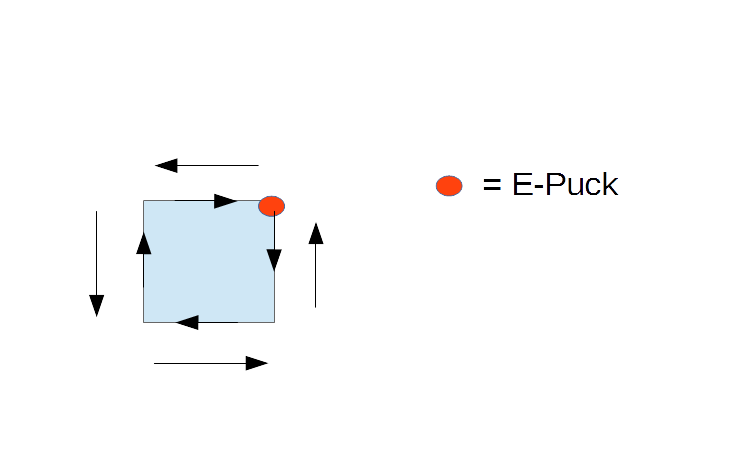
\includegraphics[width = 0.5\textwidth]{../../figures/movement_test.png} 
\caption{Movement algorithm test pattern}
\label{movement_test}
\end{figure}

Figure \ref{movement_test} shows a simple movement pattern which was used to calibrate the minimum turn distances and tested that the \textit{move\_forward()} and \textit{turn\_angle()} methods worked as intended. \\
How it works is the E-Puck starts on 1 corner of a square(here the floor of the simulator was used as it has chessboard representation) and move forwards to the other end of the square, turn 90 degrees and so on until it reaches it start point. It then turns around and follows the same pattern back to its original starting position. This tests allows the notice of odometry error in the rotations and forward movement, after a while it would turn/move to far or not far enough and thereby not reach it accurate start point. Noticing these errors allowed for calibration of the speed and distance where the algorithms will slow done the movement to minimize this error as much as possible, see section \ref{moving_forward_description} and \ref{turn_angle_description} respectively for more information on this.\\[3ex]
The test is based on the "University of Michigan Benchmark" or UMBmark\footnote{\url{http://www.cs.columbia.edu/~allen/F13/NOTES/borenstein.pdf}}.\\[3ex]

The problem with this calibration at the time was rather than using this approach to calibrate the effective wheelbase and the wheel radius at the time of this calibration the angles to turn were changed.\\
This led to rather than updating the wheelbase from  the original 0.052(which has been done in a later stage of the project. \textbf{Note: the code which can be found in Appendix B uses the updated wheelbase}.\\
Using the non-updated wheelbase it was required to change specify an angle of 100$^{\circ}$ to move 90$^{\circ}$ effectively.

\section{First results}
After the calibration process of the previous section a new program iteration was started, using the new movement and localisation algorithm in order to test the mapping and continue implementing it. \\[3ex]

This first implementation was not using the deployment pattern but rather simply following the walls, this was done so that the mapping could be tested. Rather than having an advanced wall following algorithm at this stage a simple collision avoidance algorithm was used which turned the robot by 90$^\circ$ when ever an obstacle is reached. 

\subsection{Early mapping methods and results}

\begin{lstlisting}[caption={Proximity sensor reading}]
//distance sensors array definitions
int ps_value[NUM_DIST_SENS]={0,0,0,0,0,0,0,0};
int obstacle[NUM_DIST_SENS]={0,0,0,0,0,0,0,0};
int ps_offset[NUM_DIST_SENS] = {35,35,35,35,35,35,35,35};

// obstacle will contain a boolean information about a collision
for(i=0;i<NUM_DIST_SENS;i++){
	ps_value[i] = (int)wb_distance_sensor_get_value(ps[i]);
	obstacle[i] = ps_value[i] - ps_offset[i] > THRESHOLD_DIST;
}

//define boolean for sensor states for cleaner implementation
bool ob_front =
	obstacle[PS_RIGHT_10] ||
	obstacle[PS_LEFT_10];

bool ob_right =
	obstacle[PS_RIGHT_90];

bool ob_left =
	obstacle[PS_LEFT_90];
\end{lstlisting}

The code above shows the code used at this stage of the project to detect obstacles, and set boolean values if an obstacle is detected in the direction of the  obstacle. As the test environment for this part of the project is a simple square area the turning of 90$^{\circ}$ is sufficient and no other control was needed at this stage to test the mapping. 

\begin{figure}[h]
\centering
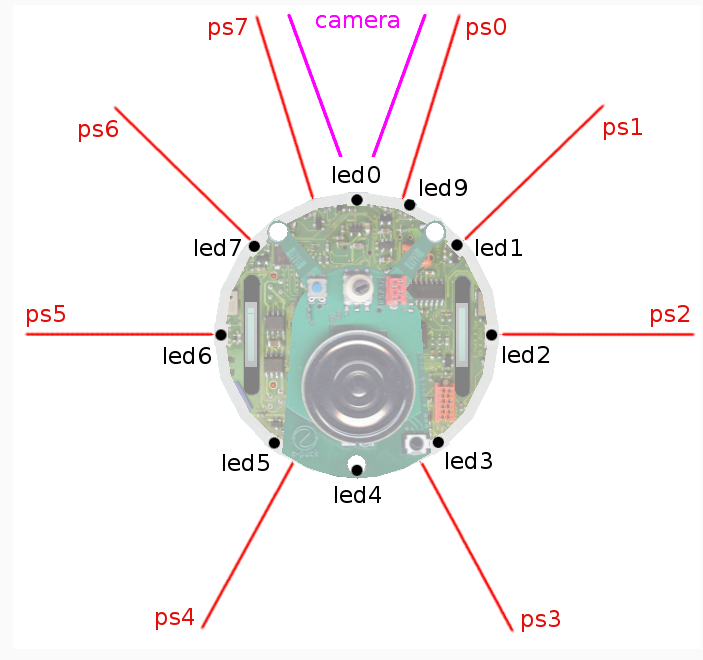
\includegraphics[width = 0.5\textwidth]{../../figures/e_puck_sensor_placement.png} 
\caption[E-Puck sensor placement]{E-Puck sensor placement\footnotemark}
\label{sensor_placement}
\end{figure}

Figure\footnotetext{Figure \ref{sensor_placement} is taken from: \url{http://www.cyberbotics.com/cdrom/common/doc/webots/guide/section8.1.html}}  \ref{sensor_placement} show the sensor placement on the E-Puck robot. Its is worth noticing that for sake of simplicity and better work flow the sensors have been renamed in the code. The new naming scheme does show which side of the robot the sensor is placed and its placement in degrees, relevant to the forward facing center of the robot. As an example the sensor ps0 in figure \ref{sensor_placement} is named PS\_RIGHT\_10 in the code since it is placed on the right side of the robot with an orientation of 10$^{\circ}$ relevant to the center.
Compared to this sensor ps5 is PS\_LEFT\_90.   \\[3ex]

The mapping algorithm used a similar approach to the obstacle detection algorithm. \\
One of the problems which were noticed at this stage was the problem of the noise simulated inside the simulator, this leads to the mapping algorithm needing a high threshold in order to map only actual obstacles, and not random noise spikes.  This however leads to the problem of the robot needing to almost be in direct contact with the obstacles in order to map them. For the mapping at this stage this was not a problem however this strongly influenced movement pattern decisions at a later stage in the implementation process, more about that in a later section.

\begin{figure}[h]
\centering
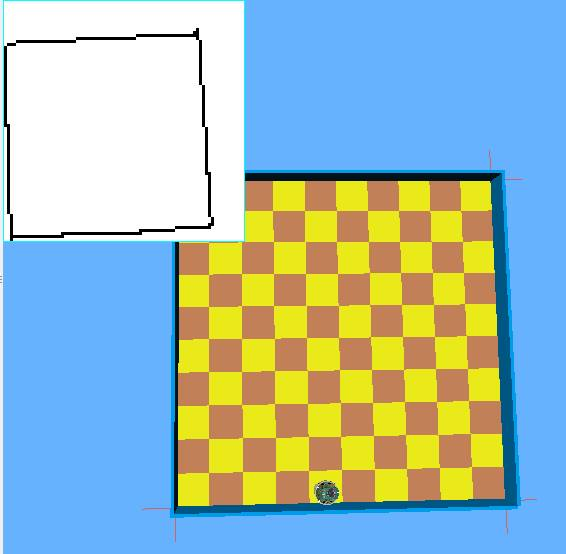
\includegraphics[width = 0.5\textwidth]{../../figures/early_map.jpg} 
\caption{Early mapping result}
\label{early_mapping_result}
\end{figure}

Figure \ref{early_mapping_result} shows clearly the strongest problems with this solution so far as well as demonstrates the need to have a good solution for  the main aspects of this project, localisation and deployment.\\
As it can clearly be seen in the figure, the localisation and movement approach were far from perfect at this stage in the project. 
While the program generates a closed  map the mapping is strongly skewed to the left side. This error was strongly based on odometry errors during turning caused by sup-optimal calibrated robot values as well as friction between the wheels and the floor.\\
At the time to movement algorithm did not update the odometry struct, and the struct were only updated once every loop iteration. \\
This was the stage of the project at the time of the mid-project demo.


\subsection{Direction control based on heading}
The approach done to fix the odometry error at this stage was done by specifying directions in which the robot is moving as north, east, south and west. 

\begin{figure}[h]
\centering
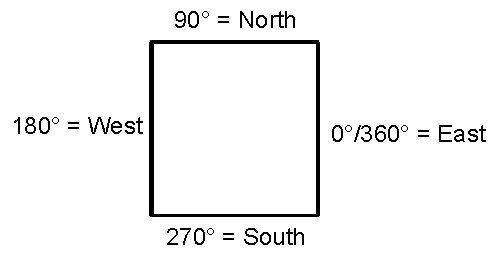
\includegraphics[width = 0.5\textwidth]{../../figures/direction_and_angles} 
\caption{Directions and their corresponding Angles}
\label{directions_and_angles}
\end{figure}

Figure \ref{directions_and_angles} does show the directions used and the corresponding angles. The directions were represented in the code by using boolean values. \\
In order to get the direction controlled movement working a number of functions needed to be created.  

\begin{lstlisting}[caption={Converting Radians to degrees}]

#ifndef M_PI
	#define M_PI 3.1415926535897932384626433832795L
#endif

#define RTOD(r) ((r) * 180 / M_PI)

/**
returns the angle in which the robot is moving
*/
int return_angle(double rad){
	double rotation;

	if(RTOD(rad) < 0){
		rotation = RTOD(rad) + 360;
	}else{
		rotation = RTOD(rad);
	}
	printf("%f\n", rotation);
	return rotation;
}
\end{lstlisting}

This function converts radians, which are used by the simulator, to degrees.This was done to make it easier to work with.
The next function uses this to check in which direction the robot is moving and set a boolean value representing a direction to \textit{true}.

\begin{lstlisting}[caption={Early check of the movement direction}]
#define ANGLE_TOLERANCE 20
#define EAST 0
#define NORTH 90
#define WEST 180
#define SOUTH 270

//direction definitions
bool north,west,south,east;

/**
set booleans for the direction the robot is moving in
*/
void check_direction(double d){
	int i = return_angle(d);
	east = false;
	north = false;
	west = false;
	south = false;

	if(EAST < i + ANGLE_TOLERANCE || EAST > i - ANGLE_TOLERANCE){
		east = true;
	}else if(NORTH < i + ANGLE_TOLERANCE || NORTH > i - ANGLE_TOLERANCE){
		north = true;
	}else if(WEST < i + ANGLE_TOLERANCE || WEST > i - ANGLE_TOLERANCE){
		west = true;
	}else if(SOUTH < i + ANGLE_TOLERANCE || SOUTH > i - ANGLE_TOLERANCE){
		south = true;
	}
}
\end{lstlisting}

At this moment the deployment pattern described in chapter \ref{Design}  was also implemented. \\
This was done by checking which direction the robot is facing when an obstacle is found in front of the robot. At this point a couple of procedures were designed for what to do for each direction. Effectively the robot is performing u-turns when ever an obstacle is found directly in front of it. 

\begin{figure}[h]
\centering
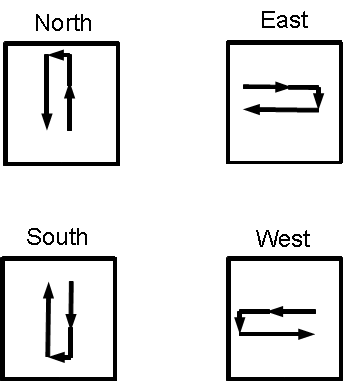
\includegraphics[width = 0.5\textwidth]{../../figures/direction_uturn_pattern} 
\caption{Directions and their corresponding U-Turn pattern}
\label{directions_uturn_pattern}
\end{figure}

The u-turn patterns shown in figure \ref{directions_uturn_pattern} effectively led the robot to move from right to left and from the top downward, there wasn't any particular reason for this, other than an uniformed pattern was needed. \\ 
The next piece of code is a snipped from the deployment loop at that time in the project. It uses the previous shown \textit{check\_direction()} as well as the \textit{controll\_angle()} method which will be shown at a later point.\\
The control angle function is used to compare the current heading with the heading specified by the general direction the robot is moving in(north/east/south/west). 
As the code snipped shows at this point the the odometry struct is still not updated during the deployment loop, and the heading is only checked and corrected in the FORWARD state of the loop. 
The \textit{turn\_right()} and \textit{turn\_left()} functions turn the robot 90$^{\circ}$.

\begin{lstlisting}[caption={Early Control loop snipped}]
double dMovSpeed = 500.0f;
double dDistance = 0.01f;
double dTurnSpeed = 100.0f;
double dTurnDistance = 0.05f;	

switch(state){
	case FORWARD:
		move_forward(dMovSpeed, dDistance);
		controll_angle(&ot);
		if(ob_front){
			state = STOP;
		}
		break;	
	case STOP:
		stop_robot();

		if(ob_front && ob_left){
			state = TURNRIGHT;
		}
		else if(ob_front && ob_right){
			state = TURNLEFT;
		}
	else if(ob_front){
		check_direction(ot->result.theta);
		state = TURNRIGHT;
	}
	break;	

	case TURNRIGHT:
		turn_right(dTurnSpeed);
		state = FORWARD;
		break;
	case TURNLEFT:
		turn_left(dTurnSpeed);
		state = FORWARD;
		break;
	case UTURN:
		if(north){
			turn_left(dTurnSpeed);
			move_forward(dTurnSpeed, dTurnDistance);
			turn_left(dTurnSpeed);
			state = FORWARD;
		}else if(south){
			turn_right(dTurnSpeed);
			move_forward(dTurnSpeed, dTurnDistance);
			turn_right(dTurnSpeed);
			state = FORWARD;
		}else if(west){
			turn_left(dTurnSpeed);
			move_forward(dTurnSpeed, dTurnDistance);
			turn_left(dTurnSpeed);
			state = FORWARD;
		}else if(east){
			turn_right(dTurnSpeed);
			move_forward(dTurnSpeed, dTurnDistance);
			turn_right(dTurnSpeed);
			state = FORWARD;
		}
		east = false;
		north = false;
		south = false;
		west = false;
		break;
	default:
		state = FORWARD;
}
\end{lstlisting}

It is worth mentioning that this approach went through a number of modifications before this state was reached. The previous modifications were done to check to optimal placement of the \textit{controll\_angle()} function. It was found to be unproductive to have the check after every turn, as it did not matter on the small distances the robot was moving in the u-turn process. \\

\begin{lstlisting}[caption={Early heading correction algorithm}, label={early_heading}]
 /**
Controll the movement angle
*/
void controll_angle(struct odometryTrackStruct *ot){
	int rotation;
	int dSpeed = 100.0f;
	int corAngle = 5.0f;

	if(RTOD(ot->result.theta) < 0){
		rotation = RTOD(ot->result.theta) + 360;
	}else{
		rotation = RTOD(ot->result.theta);
	}

	//check movement to the right(east)
	if(EAST < rotation + ANGLE_TOLERANCE){
		turn_angle(-corAngle, dSpeed);
	}else if(EAST > rotation - ANGLE_TOLERANCE){
		turn_angle(corAngle, dSpeed);
	}

	//check movement to the north
	if(NORTH < rotation + ANGLE_TOLERANCE){
		turn_angle(-corAngle, dSpeed);
	}else if(NORTH > rotation - ANGLE_TOLERANCE){
		turn_angle(corAngle, dSpeed);
	}

	//movement to the west
	if(WEST < rotation + ANGLE_TOLERANCE){
		turn_angle(-corAngle, dSpeed);
	}else if(WEST > rotation - ANGLE_TOLERANCE){
		turn_angle(corAngle, dSpeed);
	}

	//movement to the south
	if(SOUTH < rotation + ANGLE_TOLERANCE){
		turn_angle(-corAngle, dSpeed);
	}else if(SOUTH > rotation - ANGLE_TOLERANCE){
		turn_angle(corAngle, dSpeed);
	}
}
\end{lstlisting}
The code above is an early version of the algorithm which checks and corrects the heading the robot is moving in. This algorithm was used to correct the odometry error caused by the friction in the environment and the, at this stage, sub-optimal calibrated robot attributes. \\
It worked by comparing the heading the robot is heading in with the wanted heading and correcting any errors. The algorithm at this stage has some short comings such as it is not possible to turn the robot more accurate than with a 5$^{\circ}$ threshold. If the threshold was reduced to less than  5$^{\circ}$, the robot would constantly overturn. \\[3ex]

At this time it was assumed that this inaccuracy was caused by the friction simulated inside the simulator, and that this movement was as accurate as it was going to be. \\
The odometry error at this stage did improve thanks to the \textit{control\_angle()} functions, the start of the mapping was much less skewed than the previous approach, which result can be seen in function \ref{early_mapping_result} at page \pageref{early_mapping_result}. \\[3ex]

However the constant odometry error did accumulated over time, so that the location displacement became to big to able to map the environment effectively. \\
In order to try to fix the localisation error, a couple of approaches were done in order to reduce said error. Before those approaches were done some refactoring and code improvement was done.

\section{Refactoring and improvement}
In this section the refactoring and code improvements which were done at this stage of the project is described. \\
Some of the refactorings I have not addressed in this section are the movement of functions to other source files.
While it clearly is good practise to create functions at the right place in the first place, a lot of prototype functions were created in the main source files for sake of simplicity during the first functions test. These functions were later moved to other source files were they are more appropriate, and to keep the overall source file size done. 

\subsection{Deployment algorithm refactoring}
Before other approaches were tried it was decided that the deployment algorithm needed to refactored to make the code cleaner and easier. \\
The following piece of code is a snipped taken from one of the algorithm:

\begin{lstlisting}[caption={Deployment algorithm refactoring}]
double dSpeed = 500.0f;
double dDistance = 0.01f;

char no[] = "north";
char ea[] = "east";
char we[] = "west";
char so[] = "south";

case UTURN:
	if(north){
		printf("%s\n", no);
		turn_left(dTurnSpeed);
		for(it = 0;it < 5;it++){
			move_forward(dSpeed, dDistance);
		}
		turn_left(dTurnSpeed);
		north = false;
		state = FORWARD;
	}else if(south)[...]
\end{lstlisting}

As the above snipped shows the unneeded variables of \textit{dTurnSpeed} and \textit{dTurnDistance} were removed as it was decided that the algorithm, for simplicities sake, use a single value type which can easily be changed. In order to get the same amount of movement during the u-turn phase a simple \textit{for loop} is used. The same modifications as are shown in the code snipped have been done to the rest of the u-turn \textit{case}. \\
In order to improve the code further, printout statements were added to the u-turn routine as well as to the \textit{return\_angle()} function.
This needed to be done as the webots simulator does not have a debugger, so printouts were used to track to results of the algorithms.

\subsection{Deployment algorithm improvement}
\label{deployment_improvement}
The previous u-turn method did not support mapping obstacles while the u-turn was performed. As this is not optimal behavior the u-turn pattern was altered again, to support the mapping methods. 

\begin{lstlisting}[caption={U-turn improved with obstacle detection and mapping}, label={uturn_code}]
#define NUM_DIST_SENS 8 //number of distance sensors 
#define OCCUPANCE_DIST 150 //obstacle mapping threshold
double dSpeed = 500.0f;
double dDistance = 0.01f;

static int wtom(float x){
	return (int)(MAP_SIZE / 2 + x / CELL_SIZE);
}

robot_x = wtom(ot->result.x);
robot_y = wtom(ot->result.y);

char no[] = "north";
char ea[] = "east";
char we[] = "west";
char so[] = "south";

case UTURN:
	if(north){
		printf("%s\n", no);
		turn_left(dSpeed);
		for(it = 0;it < 5;it++){
			move_forward(dSpeed, dDistance);
			
			//mark cells as occupied
			wb_display_image_paste(display,background,0,0);
			wb_display_set_color(display,0x000000);
			for(i = 0;i < NUM_DIST_SENS;i++){
				if(wb_distance_sensor_get_value(ps[i]) > OCCUPANCE_DIST){
					occupied_cell(robot_x, robot_y, ot->result.theta + angle_offset[i]);
				}
			}
			wb_display_image_delete(display,background);
			background = wb_display_image_copy(display,
				0,0,display_width,display_height); 
		}
		turn_left(dSpeed);
		north = false;
		state = FORWARD;
	}else if(south){[...]
\end{lstlisting}

The above code shows how the obstacle detection and mapping were added to the u-turn \textit{case}. 
This map's the obstacles to the sides of the E-Puck while the robot moves along the side of it and proceeds to the next turn. While this mapping is not good, as it is very "spotty".

\begin{figure}[h]
\centering
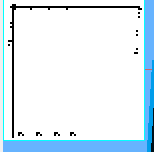
\includegraphics[width = 0.5\textwidth]{../../figures/map_results/dotted_uturn_mapping.png} 
\caption{Dotted mapping during U-Turns}
\label{dotted_uturn}
\end{figure}

Figure \ref{dotted_uturn} shows the dotted mapping which is caused during u-turns. While it is in no form a good representation of the environment it provides an outline of obstacles. The problem with this is however that because of the u-turn pattern it is needed for the robot to traverse a long each obstacle / wall in order to map them correctly. 

\section{Mapping}
In this section the mapping algorithm are shown and described. \\
The mapping algorithms are one of the key algorithms of the project, however based on code from the Webots\textsuperscript{\texttrademark} demo programs It is based on a occupancy map, which is a simple 2D map. The function used to mark a \textit{cell} of the occupancy map.\\
The code for this function can be found in Appendix A, section \ref{occupied_cell} on page \pageref{occupied_cell}.
The parameters for the function represent the X and Y coordinates as well as the rotation of the robot. These values are received from the odometry struct. 
The functions uses the Webots\textsuperscript{\texttrademark}  API to draw the cell in form of a 1x1 pixel rectangle on the display. 

\begin{lstlisting}[caption={obstacle detection and mapping}]
#define NUM_DIST_SENS 8 //number of distance sensors 
#define OCCUPANCE_DIST 150 //obstacle mapping threshold

static int wtom(float x){
	return (int)(MAP_SIZE / 2 + x / CELL_SIZE);
}


robot_x = wtom(ot->result.x);
robot_y = wtom(ot->result.y);

wb_display_image_paste(display,background,0,0);
wb_display_set_color(display,0x000000);
for(i = 0;i < NUM_DIST_SENS;i++){
	if(wb_distance_sensor_get_value(ps[i]) > OCCUPANCE_DIST){
		occupied_cell(robot_x, robot_y, ot->result.theta + angle_offset[i]);
	}
}
wb_display_image_delete(display,background);
background = wb_display_image_copy(display,0,0,display_width,display_height); 
\end{lstlisting}

The code above shows for loop which checks the value reported by each 1 of the 8 distance sensors and compare this value to the defined threshold. If the value is larger than the threshold the cell will be marked. 

\section{Refactoring of the heading correction}
In this section the refactoring of the heading correction functions is shown. 
The earlier version of this code can be seen in listing \ref{early_heading} on page \pageref{early_heading}.
The earlier version of this code snipped worked, however it was way more complex than it had to be. 

\begin{lstlisting}[caption={Refactored heading control code} ]
/**
Function to compare the current heading to the wanted heading
and fix the heading should it surpass a threshold
*/
void check_rotation(double cur_rot, double want_rot, double dSpeed){
	double dthreshold = 1; //2,0
	double diff;
	char text[] = "Correcting";
	
	if(cur_rot + 20 >= 360){
		cur_rot -= 360; 
	} 
	
	if(cur_rot > want_rot + dthreshold){
		diff = cur_rot - want_rot;
		printf("%s\n", text);
		turn_angle(diff, dSpeed);
	}else if(cur_rot < want_rot - dthreshold){
		diff = want_rot - cur_rot;
		printf("%s\n", text);
		turn_angle(-diff, dSpeed);
	}
}
\end{lstlisting}

The newer version of this function only requires parameters with defines the wanted and the previous heading rather then the need of having global boolean values to specify in which direction the robot is moving. 
This refactored approach works by comparing the wanted and current heading, an threshold is also included as the robot will never turn 100\% accurate. \\
The function also converts degrees which are above 360 $^{\circ}$, to a more sensible value. 
The code holds printout statements which allow to understand in which direction the robot thinks it is moving, which can be compared to the actual direction for testing purposes. \\[3ex]

After this function was created the threshold was calibrated in a couple of runs. The threshold which was set in the first iteration, and was gradually decreased to a value of \textit{3} at the time. The threshold value shown in the code snipped above is \textit{1}, this value was reached by recalibrating the turning and movement functions, more about that can be found in section \textbf{FIXME(enter section number)}.

\section{New approach tried and implemented}
In this section the different approaches which were tried at this development stage are described. While not all approaches were successful not every aspect of them was discarded.

\subsection{Dynamic U-Turn approach}
At this point in the development process a new approach for turning the robot in the U-turn routine was tested. The idea was to change from using a static turning command \textit{turn\_left(dSpeed)}, which can be seen i code snipped \ref{uturn_code} on page \pageref{uturn_code}, to a more dynamic approach. \\
In this new dynamic approach the angle to turn was calculated from the current rotation and the wanted angle.

\begin{lstlisting}[caption={Code snipped of the new approach}, label={newApproach}]
double cur_rot;
	
else if(south){
	printf("%s\n", so);
	turn_right(dTurnSpeed);
	for(it = 0;it < 5;it++){
		move_forward(dTurnSpeed, dDistance);
		//mark cells as occupied
		wb_display_image_paste(display,background,0,0);
		wb_display_set_color(display,0x000000);
		for(i = 0;i < NUM_DIST_SENS;i++){
			if(wb_distance_sensor_get_value(ps[i]) > OCCUPANCE_DIST){
				occupied_cell(robot_x, robot_y, ot->result.theta + angle_offset[i]);
			}
		}
		wb_display_image_delete(display,background);
		background = wb_display_image_copy(display,0,0,display_width,display_height);
	}
	odometry_track_step(ot);
	cur_rot = return_angle(ot->result.theta);
	turn_angle(cur_rot - 90, dTurnSpeed);
	//turn_left(dSpeed);
	south = false;
	state = FORWARD;
}else if(west)[...]
\end{lstlisting}

The code in listing \ref{newApproach}, is a snipped from the U-turn routine. \\
However this approach did not work out as the robot always turned to far. Rather than getting stuck on this new approach, it was discarded and work was resumed with the old, static version of the code where the robot simply always turns 90$^{\circ}$. \\

\subsection{Stop on corner detection}
At this stage it was noticed that some of the existing odometry error existed because the robot did not stop when an obstacle, like a corner was encountered in the U-turn routine. 
What actually happened is that the robot wheels kept turning, increasing the encounter values, which let to wrong odometry calculations. \\
To fix this problem corner detection was added to the algorithm. 
It is worth noting at this point that rather than only corner detection, general obstacle detection should have been added. However, as it described in chapter 4, the program was only ever tested in the same environment during development which let to many of the problems encountered in the tests. 
The reason that only corner detection was added at this point was because it was known that the only obstacle which will be encountered in the U-turn routine are going to be corners, so no other type of obstacles was even considered.\\[3ex]

In the first iteration of this approach is corner detection was added \textbf{bellow} the section of code which mark's cells as occupied. Test runs quickly showed that it works better \textbf{before} said section, so the corner detection was moved.\\
The snipped shown in listing \ref{corner-uturn} is the final version with the corner detection above the cell marking section.

\begin{lstlisting}[caption={Corner detection added to the U-turn routine}, label={corner-uturn}]
if(north){
	printf("%s\n", no);
	turn_left(dSpeed);
	for(it = 0;it < 5;it++){
		if((ob_front && ob_right) || (ob_front && ob_left)){
			state = STOP;
			break;
		}
		move_forward(dSpeed, dDistance);

		//mark cells as occupied
		wb_display_image_paste(display,background,0,0);
		wb_display_set_color(display,0x000000);
		for(i = 0;i < NUM_DIST_SENS;i++){
			if(wb_distance_sensor_get_value(ps[i]) > OCCUPANCE_DIST){
				occupied_cell(robot_x, robot_y, ot->result.theta + angle_offset[i]);
			}
		}
		wb_display_image_delete(display,background);
		background = wb_display_image_copy(display,0,0,display_width,display_height); 
	}
	turn_left(dSpeed);
	north = false;
	state = FORWARD;
}else if(east){[...]
\end{lstlisting}

\subsection{Added odometry update function to the movement algorithm}
Until this stage the odometry values were only updated every control loop iteration. \\
In order to increase the number of odometry updates, which needed to be done in order to make the localisation more accurate, the odometry update function needed to be called more often then just once every iteration.
This was done in an approach to reduce the overall odometry error  by updating the \textit{odometry struct} more often, before odometry errors has a change to accumulate further. \\[3ex]

In order to implement this the odometry updated function was added to the \textit{move\_forward()} function. 
The code which can be found in Appendix B section \ref{moving_forward_code} on page \pageref{moving_forward_code} is the version of the code with the odometry update function added to it. \\
While this updated function did not show any significant decrease of the localisation error, it was kept as updating the odometry functions as often as possible is helps decreasing the overall localisation error. 

\section{Recalibration of the movement algorithms}
The approaches described in the previous section allowed to reduce the overall odometry error by small degrees, however not entirely remove it. \\
Research was done of how to reduce the odometry error and a paper written by Johann Borenstein and Liqiang Feng was found \cite{Borenstein1996Measurement}.\\

In this paper \textit{Borenstein et al.} described why and how odometry error are generated and how to minimise them by having a good calibrated robot. 
They showed ways of calibration the parts of the robot which cause odometry error when turning and driving forward, the \textit{wheelbase} and the \textit{wheel diameter}. 
They also described what kind of errors can be generated by not having an good calibrated robot.\\
The information displayed in the paper will not be repeated in this document, however the main aspects of the problems and of the calibration will be discussed.\\

There are 2 types of errors which are discussed in the paper, \textit{systematic errors} and \textit{non-systematic errors}. \textit{Systematic errors} are caused(or prevented) by values which can be fixed in software. Such error sources are: \\
\begin{itemize}
\item unequal wheel diameters
\item misalignment of wheels
\item limited encoder resolution
\item limited encoder sampling rate
\end{itemize}
Just to mention some. \\
\textit{Non-systematic errors} are caused by environmental and physical problems with the problems.
Such error sources are:\\
\begin{itemize}
\item slippery floors
\item over-acceleration
\item fast turning(skidding)
\item nonpoint wheel contact with the floor
\end{itemize}
Just to mention some.\\
\textit{Non-systematic} errors can be in this case be avoided because it known that the floor in the simulator is not slippery and there is also always wheel contact to the floor. To reduce the possibility of over-accelerating and skidding the moving and turning speed has been reduced in the program.\\
However \textit{systematic errors} are more grave then \textit{non-systematic}, this is because they accumulate constantly.\\[3ex]

\subsection{Wheelbase and Wheel diameters}
The paper describes that the 2 most notorious  error sources are \textit{unequal wheel diameters} and \textit{uncertainty about the effective wheelbase}.\\
Unequal wheel diameters are created in reality because of inaccuracy of the produced rubber wheels in robots. It is known that the wheels of the virtual E-Puck representation have unequal wheel diameters, this was discovered during the tutorials done in the very beginning of the development process.\\
For the duration of the entire development process up to this point, the values provided in these tutorials have been used. However in the beginning of the development process when the turning algorithm was implemented, a value of 100$^{\circ}$ was needed to turn 90$^{\circ}$.\\
This was because of uncertainty about the wheelbase, this however was not realised until this point.\\[3ex]

In order to describe what kind of errors uncertainty's about the wheel diameters and the wheelbase cause, the paper is going to be summarized. \\[3ex]

\textit{Unequal wheel diameters}:\\
While unequal wheel diameters do not cause an orientation error while turning, they will cause an curved movement path rather than a straight path.\\
The error can be denoted as :\\
$E_{d} = D_{R} / D_{L}$\\
Where $D_{R}$ are $D_{L}$ are the \textit{actual} wheel diameters. The \textit{nominal} ratio between the wheel diameters is of course 1.00\cite{Borenstein1996Measurement}.\\
The values of the E-Puck wheels in the simulator are:\\
$D_{R} = 0.0404 = 40.4mm$\\
$D_{L} = 0.0416 = 41.6mm$\\
These values have been taken from the Webots\textsuperscript{\texttrademark} tutorials and been confirmed in the later calibration process.\\

\textit{Uncertainty about the Wheelbase}:\\
The wheelbase is defined as the distance between the drive wheels of the robot. This wheelbase must be known in order to compute the correct amount of encoder steps each motor must take in order to turn a certain amount of degrees.
Uncertainty about this wheelbase can cause inaccuracy while turning, but does not have any effect on straight movement.\\
This error can be denoted as:\\
$E_{b} = b_{actual} / b_{nominal}$\\
Where $b$ is the wheelbase of the vehicle\cite{Borenstein1996Measurement}.\\
The value of the wheelbase provided by the Webots\textsuperscript{\texttrademark} tutorials is:\\
$0.052 = 52mm$\\
However the calibration process which is shown later shows that actual wheelbase is:\\
$0.058 = 58mm$\\
Which is an significant amount of uncertainty.\\

\begin{figure}[h]
\centering
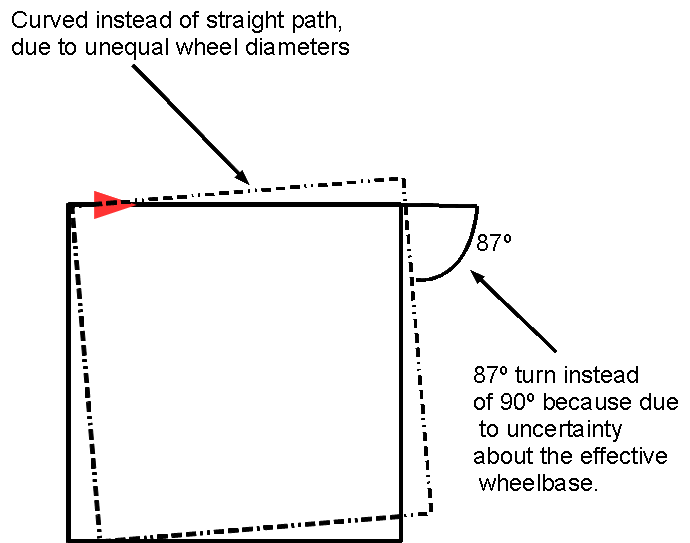
\includegraphics[width = 0.5\textwidth]{../../figures/sys_odometry_error} 
\caption{The effect of systematic odometry errors}
\label{sys_error}
\end{figure}

The paper by \textit{Borenstein et al.} describes the main danger about uncertainty of either the \textit{wheel diameters} or the \textit{wheelbase} as that modifying one of them can cause the other value to seem calibrated as well. This can be caused by using an \textit{unidirectional} square path as a benchmark test, which is what have been done in the beginning of this project, see \ref{mov_calibration} on page \pageref{mov_calibration} for more information. \\
The danger with this approach is that it is easy to analyse the odometry error being caused by either the wheel diameters, a slightly curved movement path, or the wheelbase which would caused over or under turning. \\
If only an unidirectional calibration approach is done either of these errors can be "fixed" by modifying either the wheel diameters or the wheelbase and the result would show a "correct" result.
For example if the actual movement path is as displayed by the dotted line in figure \ref{sys_error}, the movement error could be "fixed" by modifying the wheelbase which would led to robot turn, say 93$^{\circ}$, which would cause the path to appear correct. By doing that the path will look correct and thereby the robot calibrated, but in reality the robot overturns in order to compensate for the curved movement path.\\
However this will lead to increased odometry errors as the robot will appear to turn accurately but the odometry error is in reality caused by the uncertainty about the wheel diameters which leads to a curved movement path. Of course this can also happen the other way around.\\


\subsection{Bidirectional Square Path calibration: "UMBmark"}
As the preceding section shown an \textit{unidirectional} square path is unsuitable for testing odometry performance as it can easily conceal 2 mutually compensating odometry errors.\\
To overcome this problem, the paper introduces a \textit{bidirectional} square path experiment, called the \textit{University of Michigan Benchmark} or for short \textit{UMBmark}. 
In this experiment the robot moves both clockwise and counter clockwise in a square path. This way it easily shows the concealed odometry error which is caused when the robot has been calibrated by only an unidirectional approach.\\

\begin{figure}[h]
\centering
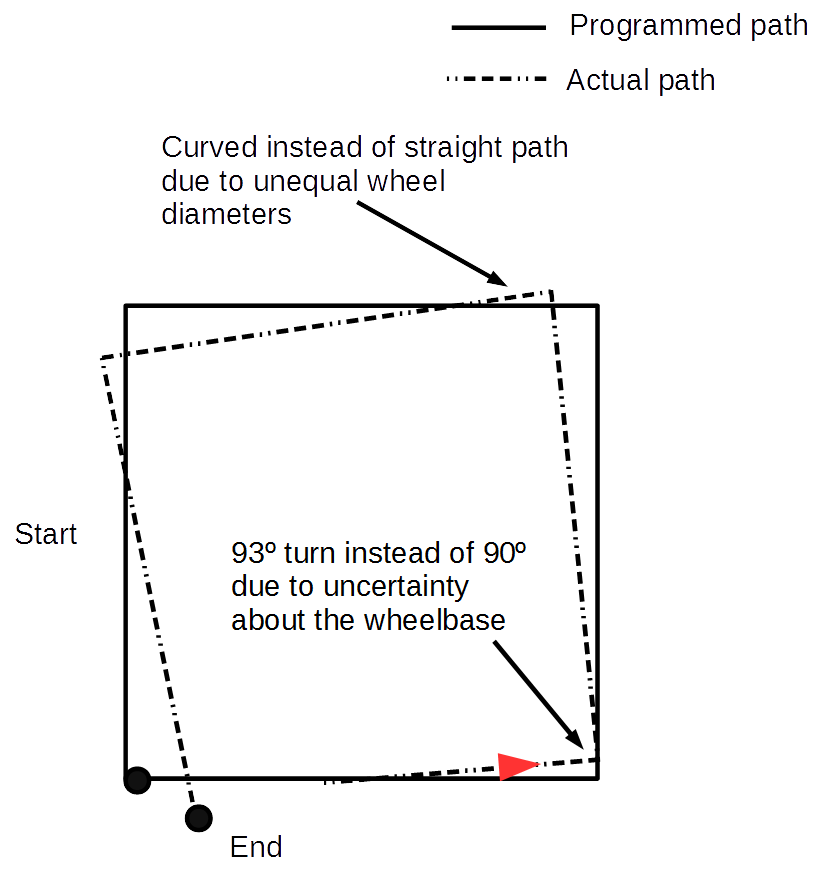
\includegraphics[width = 0.5\textwidth]{../../figures/unidirectional_error} 
\caption{The odometry error when the unidirectional path is performed in the opposite direction}
\label{unidirectional_error}
\end{figure}

Figure \ref{unidirectional_error} shows the result of running a robot which has been "calibrated" with the \textit{unidirectional} approach in the opposite direction. It shows clearly the short comings of such "calibration" as it now overturns in addition to the curved movement path.\\[3ex]

The paper describes methods which allow of accurate mathematical solutions to the given problems. But since the  Webots\textsuperscript{\texttrademark} simulator does not posses inbuilt tools to measure robot movement accurately no measurements can be taken to which would allow to follow this procedure.\\
What has been done to calibrate the E-Puck robot is to implement the UMBmark functions inside the project and run them, altering the \textit{wheel diameter} and \textit{wheelbase} values over time and compare the results.\\


\begin{lstlisting}[caption={The UMBmark experiment procedure}, label={UMBmark}]
double dSpeed = 300.0f; //movement speed
double dDistance = 0.5f;  //movement distance of 1 square. These distances have been changed over time

/**
University of Michigan Benchmark
*/
void UMBmark(double dSpeed, double dDistance){	
	//move the robot clockwise and counterclockwise 
	measure_clockWise(dSpeed, dDistance);
	
	measure_CounterClockWise(dSpeed, dDistance);
	
	stop_robot();
} 
/**
Function to measure the movement accuracy by driving
a clockwise square.
This is part of the UMBmark algorithm
*/
void measure_clockWise(double dSpeed, double dDistance){
	int i, j;
	
	for(i = 0;i < NUMTOURNAMENTS; i++){
		for(j = 0;j < 4;j++){
			move_forward(dSpeed, dDistance);
			turn_right(dSpeed);
		}
		wb_robot_step(TIME_STEP);
	}
}  

/**
Function to measure the movement accuracy by driving
a counter-clockwise square.
This is part of the UMBmark algorithm
*/
void measure_CounterClockWise(double dSpeed, double dDistance){
	int i, j; 
	
	//turn the robot right for moving the same square counter clock wise
	turn_right(dSpeed);
	
	for(i = 0;i < NUMTOURNAMENTS;i++){		
		for(j = 0;j < 4; j++){
			move_forward(dSpeed, dDistance);
			turn_left(dSpeed);
		}
		wb_robot_step(TIME_STEP);
	}
} 
\end{lstlisting}

Listing \ref{UMBmark} shows the code used for the UMBmark algorithm which is implemented inside the project. The start values are to move with a speed of \textit{300}, which is an acceptable speed as well as moving a distance of \textit{0.5}, which equals FIXME(check how many square this equals).\\
As a reminder the start values for the wheel diameters are:\\
$D_{R} = 0.0404 = 40.4mm$\\
$D_{L} = 0.0416 = 41.6mm$\\
Where $D_{R}$ represents the right wheel diameter and  $D_{L}$ the left wheel.\\
The value of the wheelbase is:\\
$0.052 = 52mm$\\ 

Firstly the amount of degrees which the robot turns when the \textit{turn\_left()} and \textit{turn\_right()} methods has been set from 100$^{\circ}$ to 90$^{\circ}$. The simulation was then been run 10 time times per test iteration to assure that the robot movements are not caused by random effects.\\
Between each iteration either of the wheel diameter and wheelbase values has either been decreased or increased in the simulation then been run for another 10 times. After each test iteration of 10 runs the value was either set back to its original value of the odometry error increased or if the error decreased the value was further changed. \\
At a later point when the odometry error seamed resolved multiple values were changed, in order to assure that they are correct. \\
The resulting result was that the wheel diameters are correct however the wheelbase value was updated from:\\
$0.052 = 52mm$\\ 
to:
$0.058 = 58mm$\\ 
As it is simple to check the current calibration for a curved movement error the robot was moved the whole length of the simulation range to confirm that the movement path is indeed straight and not curved, which it was. This was done to recheck that the result from the UMBmark calibration are correct. \\[3ex]

The paper suggest using larger movement patterns, where available, in order to check to correctness of the calibration. As this was easily done in the simulator the square was increased from 1x1 floor square to 2x2 and then 4x4. The results were largely the same, however by a square size from 4x4 the robot did not move full 4 squares. This shows that the squares on the floor, which until now have been expected to be FIXME(Check these values) 0.5 in code or equal to FIXME(add size), are not exactly that value but something close to it. \\
Because of the rest amount of time available was not big by the time of this calibration process the calibration results from 1x1 and 2x2 square paths have been deemed sufficient, rather than running multiple experiments trying to figure out the exact size of the squares. \\

\section{Reference point approach}
After the E-Puck values have been calibrated with the method described in the preceding section, the movement improvement has been checked in the development environment. \\

\begin{figure}[h]
\centering
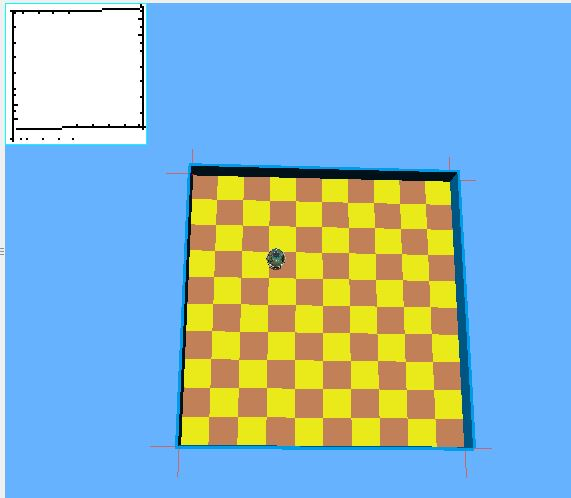
\includegraphics[width = 0.5\textwidth]{../../figures/odometry_error} 
\caption{Improved mapping with the calibrated robot, but the localisation error still persists}
\label{odometry_error}
\end{figure}

Figure \ref{odometry_error} shows the mapping result generated with the calibrated movement.\\
It shows that program is now able to generated a map of the environment with straight walls, compared to the much more skewed wall result which were generated before. 
FIXME(Rollback github repo and add screenshot about it)\\

However it is not entirely perfect at this stage as an localisation error still persists, as the robot while mapping the lower wall maps it inside the wrong place. \\
This is the result of noise generated inside the environment as well the nature of odometry calculations.
Odometry is always, in best case, an estimate of the localisation, this combined with noise and friction inside the simulator environment caused the robot to never turn 100\% accurate. \\
The algorithms implemented until this point, which compare the heading of the robot and turn it to fit the wanted heading as well as the recalibrated movement algorithms made huge improvements to the robots movements.\\
But still a minimal odometry error persists, which accumulates over time and cause the odometry error which can be seen in figure \ref{odometry_error}. \\[3ex]

At this point the use of reference points was considered in order the fix the localisation problem.\\
The approach taken for the reference point was to use the corners of the room as reference points.
This would be achieved by creating new functions and a \textit{struct }which use the already existing corner localisation implemented inside the U-Turn routine and save the X and Y coordinates the robot has calculated. 
That way the robot can reset it's X and Y coordinates to the coordinates previous saved inside the struct once the same reference point is reached again.\\
In the following subsections the functions created for this approach are being described.

\subsection{Reference point struct}
\label{ref_struct_description}
The code for the reference point struct can be found in appendix B section \ref{ref_struct_code} on page \pageref{ref_struct_code}.\\
To accommodate the idea of using the corner as reference points as structure was created which hold 4 members: \textit{lower\_left}, \textit{lower\_right}, \textit{upper\_left} and \textit{upper\_right}, where each member represents a corner of the environment. \\
Every member of the struct holds 2 float variables, which represent the X and Y coordinates of the corner.
It is worth noting that this struct has been created in correlation with the development environment which is a simple room with 4 corners.

\subsection{Checking for reference points}
\label{ref_check_description}
The code for this function can be found in appendix B section \ref{ref_check_code} on page \pageref{ref_check_code}.\\
It is called every time the main control loop finds a corner. \\
This function represents the major part of the algorithm. It compares the distance sensor data to specify which corner has been encountered and after that controls if the corner has already been saved.
Should that not be the case the function \textit{set\_reference\_point()} is called. This function will save the reference point to the struct, and is described further down. \\
If the found corner is already set as a reference point and the robots positions is within a threshold of 20, the function will reset the robots current X and Y coordinates to the values stored inside the struct. The threshold is used to make sure that the it is the same corner, rather than an unset corner inside an environment with more than 4 corners. \\
This function hold print statements which state at which corner the robot thinks it is resetting and to what coordinates. 

\subsection{Saving a new reference point}
\label{ref_save_description}
The code for this function can be found in appendix B section \ref{ref_save_code} on page \pageref{ref_save_code}.\\
This function is used to save the coordinates of a corner to the reference struct and thereby saving it as a reference point. \\
When the function \textit{check\_reference\_points()} encounters a new corner which has not been set this function is called. It requires a pointer to the odometry struct to be able to read the current X and Y coordinates of the robot, as well as an integer value which represents which corner has been found. This is done in the function \textit{check\_reference\_points()} and then simply passed as a parameter to this function. \\
This function then simply read the current coordinates and saves them to the corresponding values of the reference struct.\\
This function also holds print statements to show when the algorithm saves a new corner and with what coordinates.

\section{Mapping results using the new reference point approach}
After implementing the reference point approach discussed in the previous section the mapping results improved massively.\\
Figure \ref{ref_result} shows the mapping results after the reference point algorithm has been implemented. \\
The improve can easily be seen by comparing figure \ref{odometry_error} on page \pageref{odometry_error} with the result of figure \ref{ref_result}.

\begin{figure}[h]
\centering
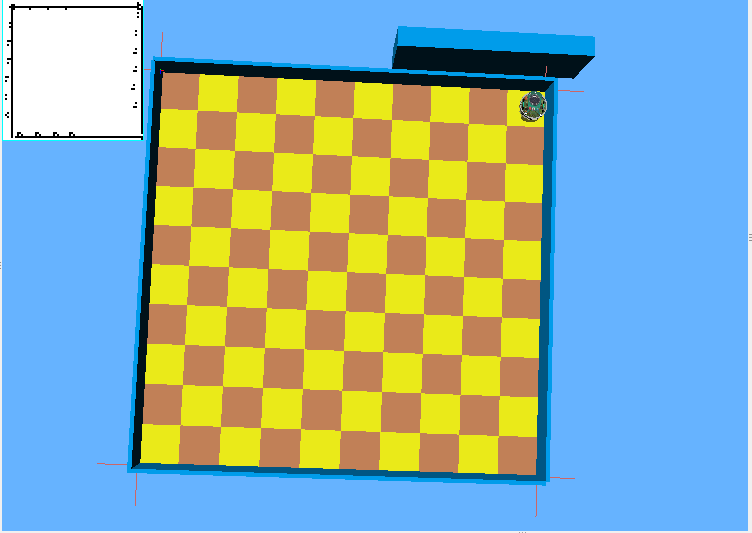
\includegraphics[width = 0.5\textwidth]{../../figures/map_results/result_room1_empty.png} 
\caption{Results after implementing the reference point algorithm}
\label{ref_result}
\end{figure}






 




